\section{Attempt to extract W+jets shape from data using ``mixed events''}

\subsection{Attempt in W+jets events}

The shape of the W+jets background is modeled from MC.  In hopes of 
obtaining a data driven shape we explored mixing jets from events to 
produce the W+jets shape template.  Although this method doesn't do an 
adequate job of describing the shape we document it here.

Using the W+jets MC, we took the W and leading jet from one event
and the second leading jet from another event.  We calculated the dijet
mass for the new paring and ensured that the new pairing satisfied all 
of our analysis level selection.  We stored the new $m_{jj}$ along with 
the $R_{jj}$ in a histogram for use as a template.  The 
results of this initial attempt are shown in Fig.~\ref{fig:mjj_mixed}.

\begin{figure}[!h]
\begin{center}
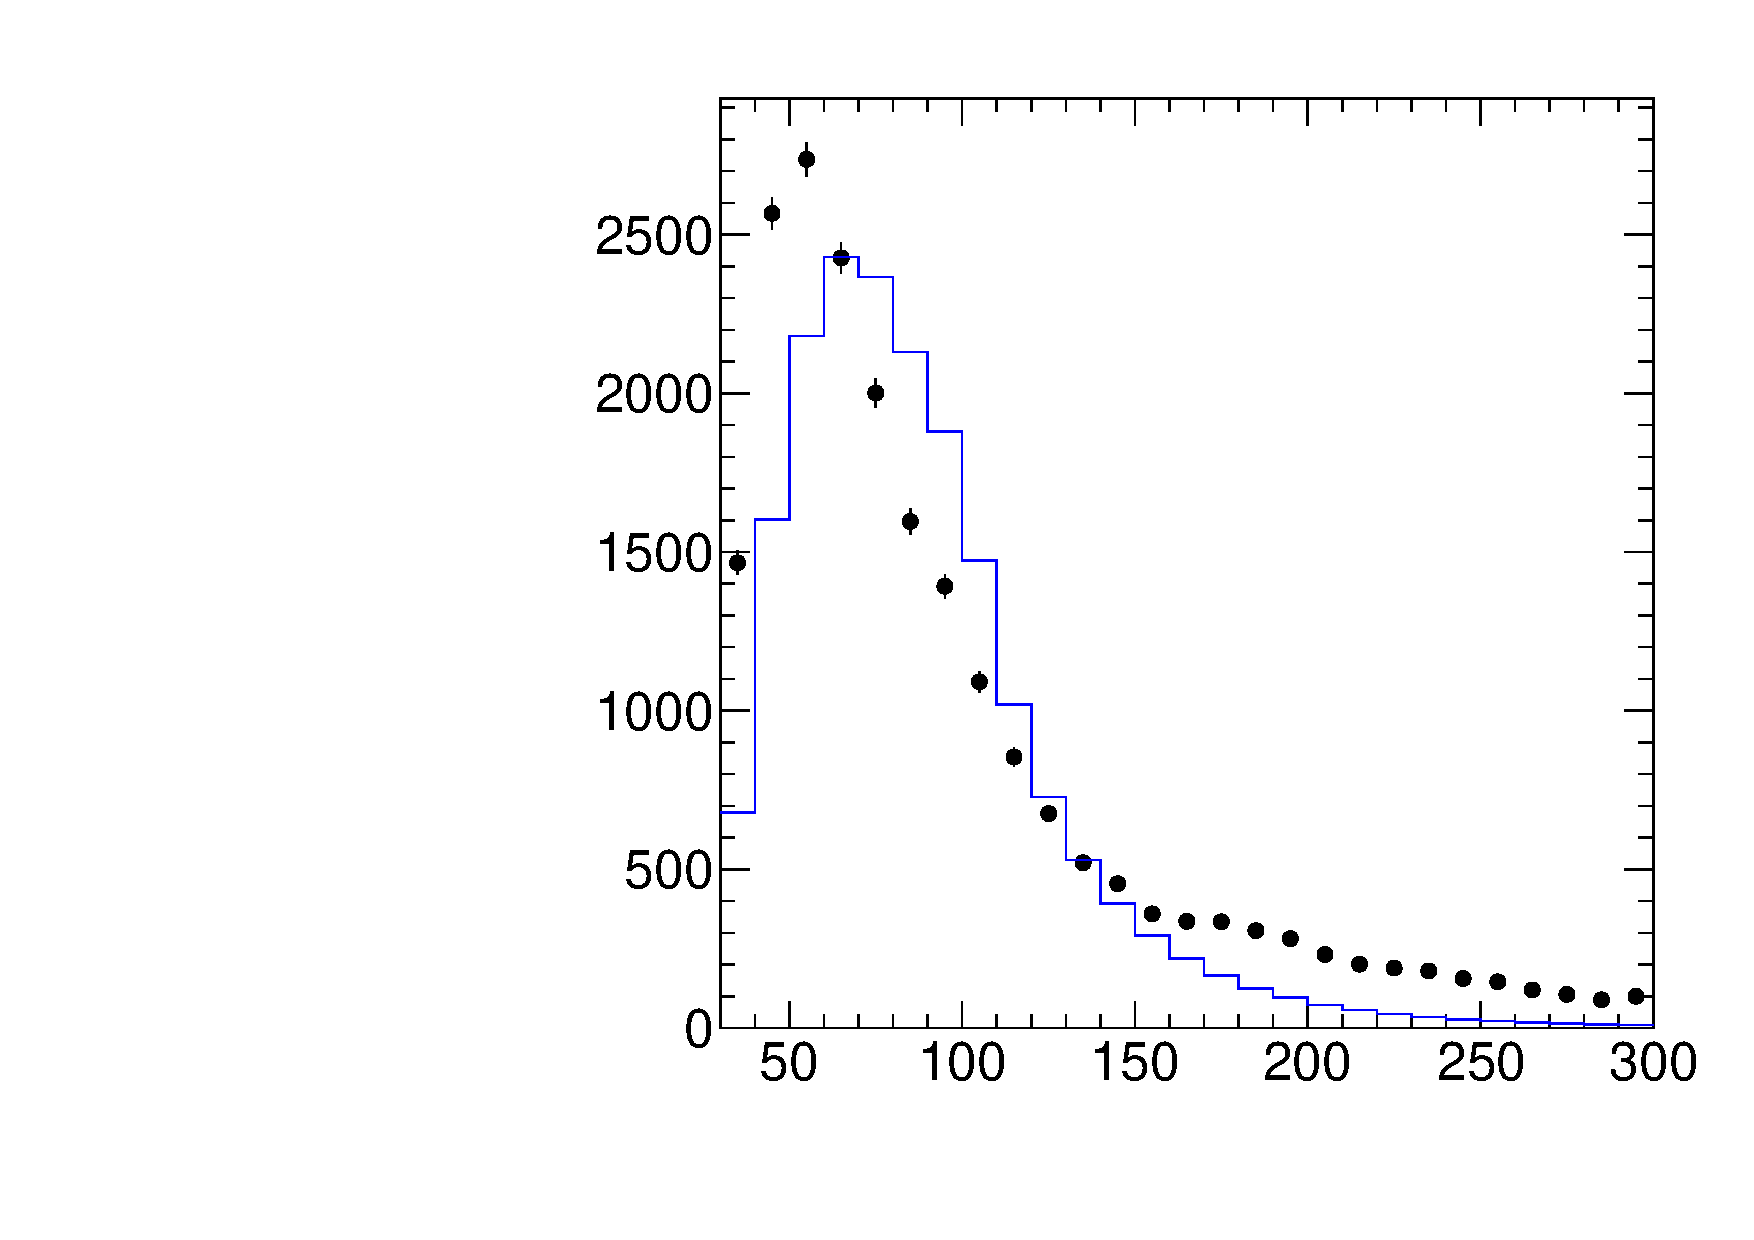
\includegraphics[width=0.6\columnwidth]{figs/mixed_Mjj}
\end{center}
\caption{\label{fig:mjj_mixed}Di-jet mass spectrum for W+jets where
the points are the correlated MC and the histogram is the mixed MC.  The
normalization excludes the first 5 bins.}
\end{figure}

With a hope of improving the agreement of the shape, we weighted the 
mixed distribution using the $R_{jj}$ from the correlated MC.  The 
$R_{jj}$ distributions are shown in Fig.~\ref{fig:Rjj_mixed}.  This led 
to better agreement as shown in Fig.~\ref{fig:mjj_mixed_w}, but the two 
shapes were still not sufficiently similar to declare closure and pursue 
this further.  This method failed because the 
\pt of the two jets is not uncorrelated as it is by construction
in this mixed scenario.

\begin{figure}[!h]
\begin{center}
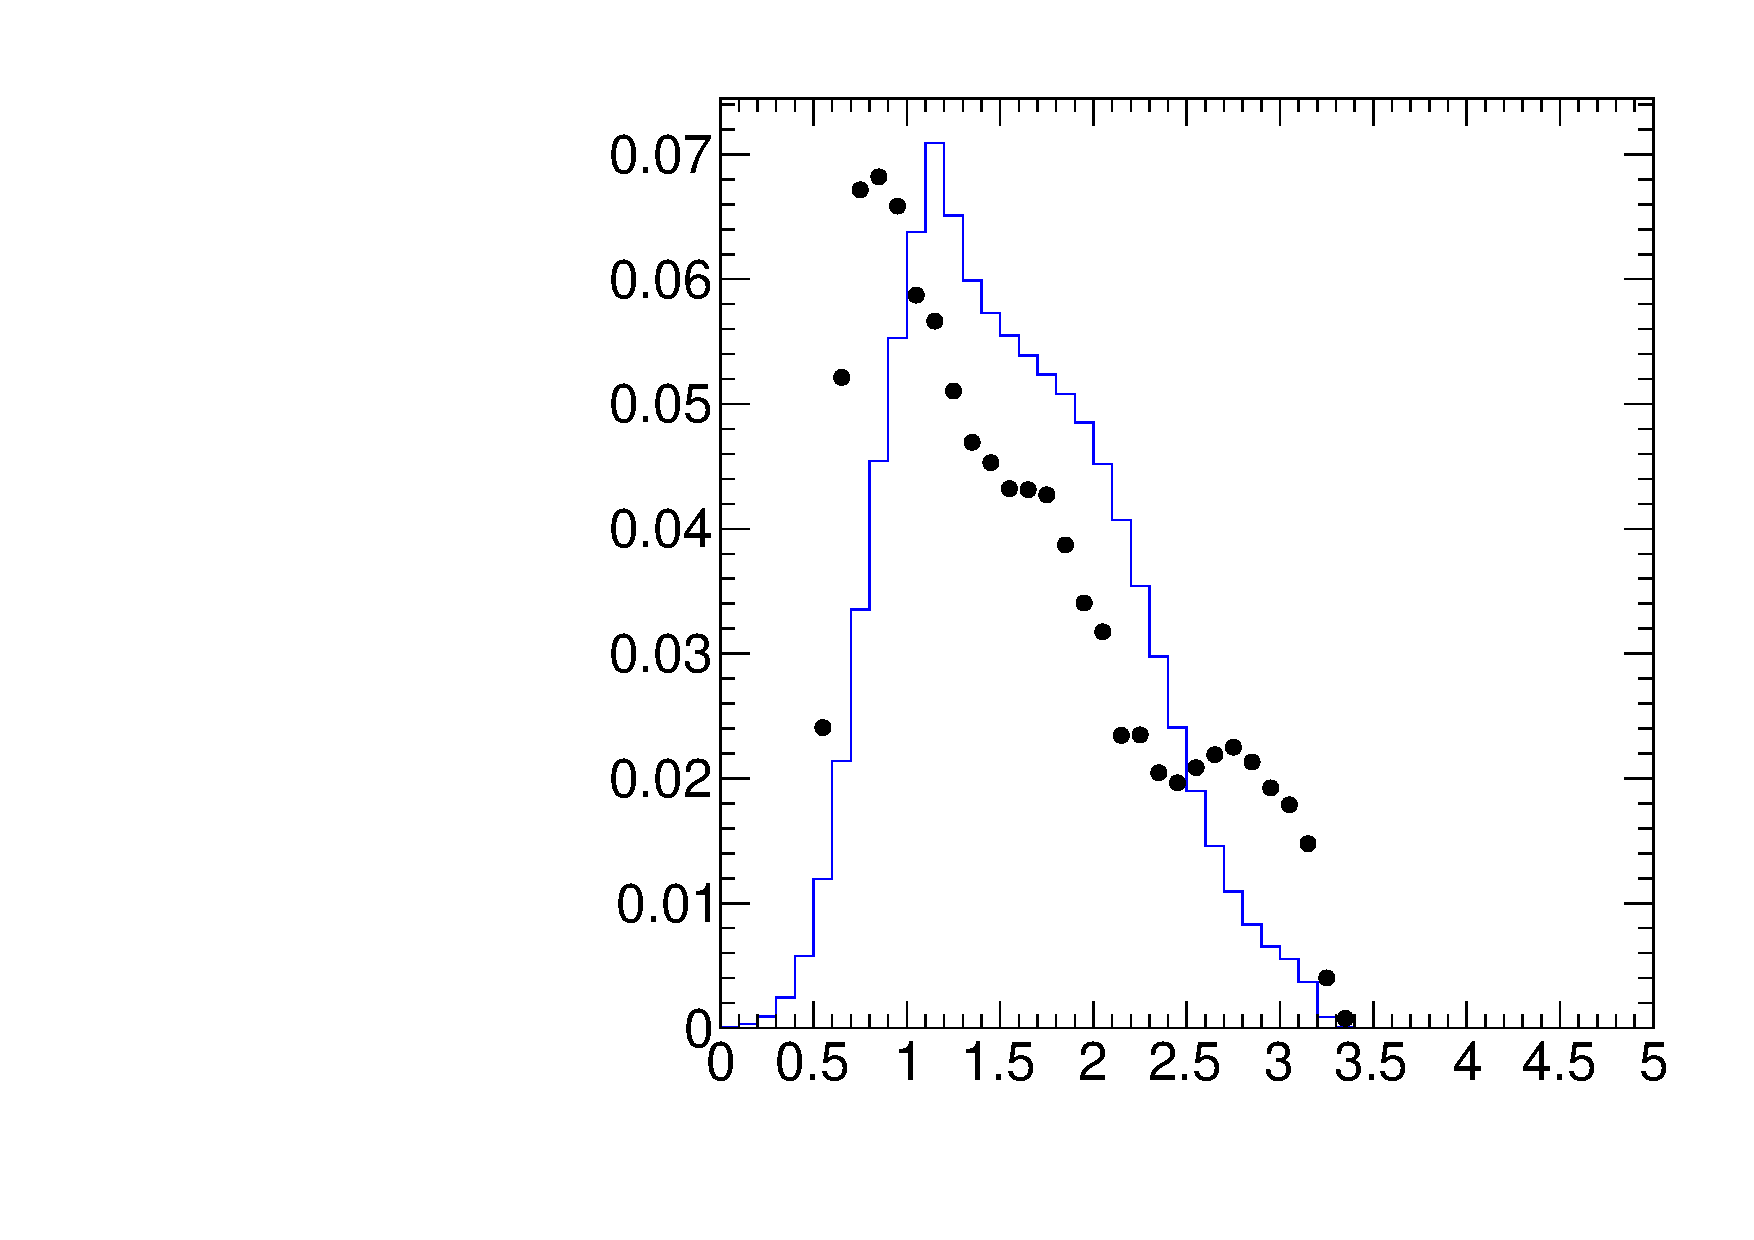
\includegraphics[width=0.6\columnwidth]{figs/mixed_Rjj}
\end{center}
\caption{\label{fig:Rjj_mixed}$R_{jj}$ for W+jets where
the points are the correlated MC and the histogram is the mixed MC.}
\end{figure}

\begin{figure}[!h]
\begin{center}
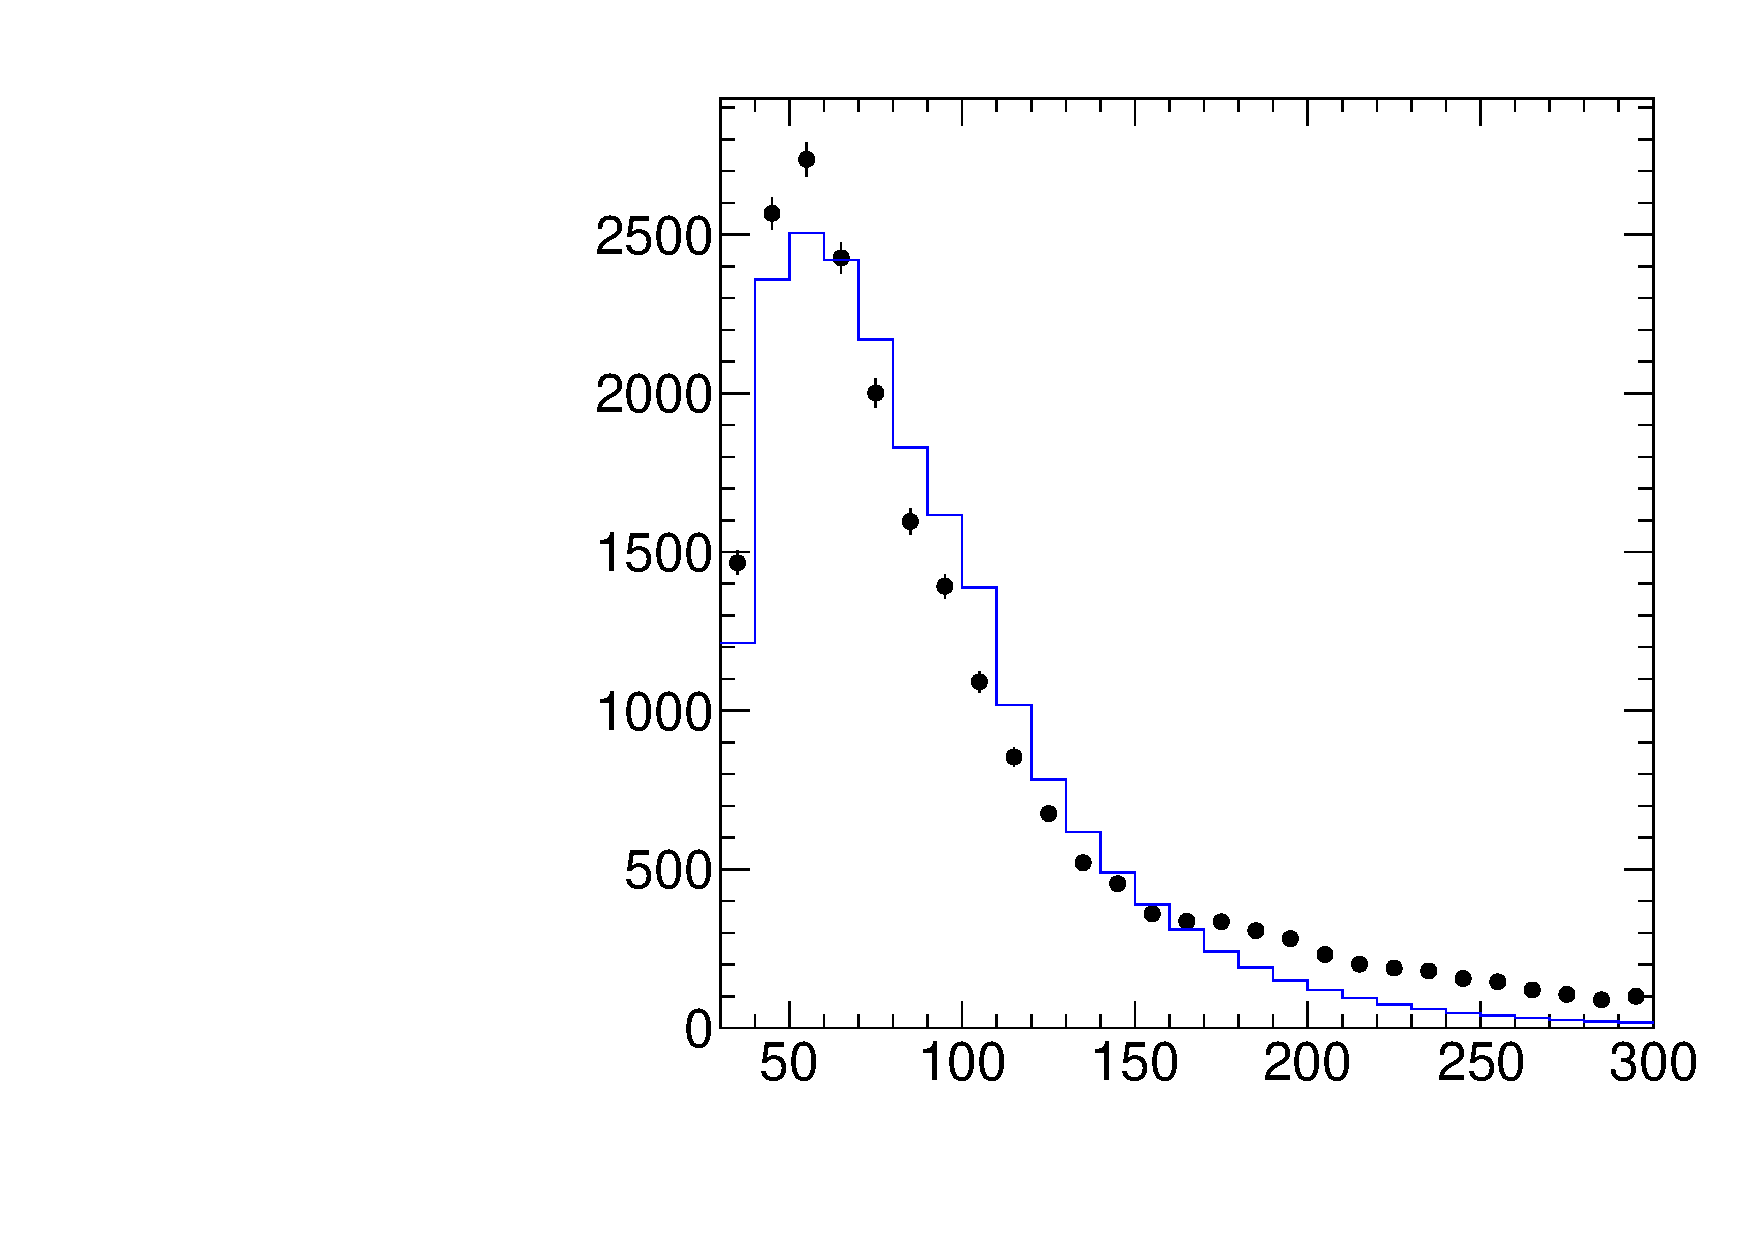
\includegraphics[width=0.6\columnwidth]{figs/mixed_Mjj_weighted}
\end{center}
\caption{\label{fig:mjj_mixed_w}Di-jet mass spectrum for W+jets where
the points are the correlated MC and the histogram is the mixed MC.  The 
normalization excludes the first 5 bins.  The mixed spectrum has been 
weighted using the $R_{jj}$ distribution from the correlated MC.}
\end{figure}

\clearpage

\subsection{Working example (Bi-Event Subtraction Technique (BEST))}


In W + jets events, the dijet mass spectrum in mixed events did not seem
to model combinatorial background very well. The same method, however,
does work in other event selections. This subsection demonstrates that
multijet mass spectrums in mixed events well model combinatorial
background in top pair production events in the framework of
\textit{Bi-Event Subtraction Technique} (BEST) \cite{Dutta:2011gs}.
The detail of the analysis is described in \cite{CMS-AN-2011-396}.

The BEST concerns three invariant mass distributions of multijets: the
\textit{same event distributions}, the \textit{bi-event distributions},
and the \textit{BEST event distributions}. The same event distributions
are the usual invariant mass distributions of multijets in the same
events. They might include signal resonances as well as combinatorial
background. The bi-event distributions are the invariant mass
distributions of multijets in different events, which are called
\textit{bi-events}. In bi-events, no resonances can be expected because
the momenta of jets in bi-events are uncorrelated. After appropriately
normalizing the bi-event distributions, they are subtracted from the
same event distributions. The resultant distributions are called the
BEST event distributions, which approximate the invariant mass
distributions of resonating multiple jets.

Fig. \ref{153631_13Aug11} shows the same event, bi-event, and the BEST
event distributions for dijets. The events were online triggered by
\textit{HLT\_IsoMu24\_v*}. Later offline the events were further
selected to choose top-antitop quark pair production events in which a
top quark decays to a bottom quark, a muon, and a muon neutrino while
the other top quark decays fully hadronically to three jets with one jet
b-tagged \cite{CMS-AN-2011-396}. In the figure, a good agreement of the
tails of the same event and bi-event distributions are observed. In
addition, the peak can be clearly seen at around the mass of the W boson
(80.4 GeV). This tail agreement and the W boson mass peak indicate that
the BEST properly functions on this selection of events.

\begin{figure*}[!h]
 \begin{center}
  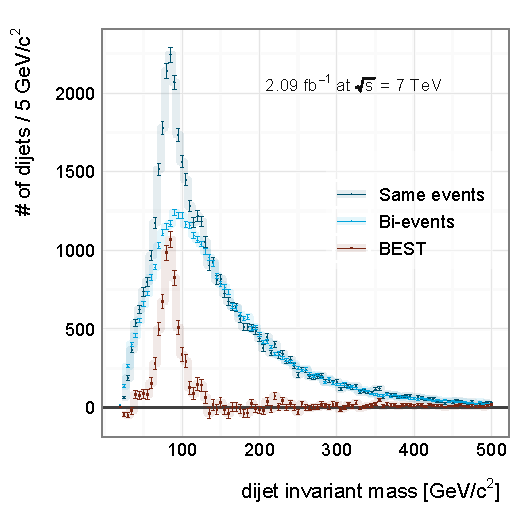
\includegraphics[scale=1.]{figs/best/c110506_s0102_g001_01}
 \caption{The
invariant mass distributions of dijets in the same events, bi-events,
and BEST events in 2.09 fb${}^{-1}$ of data. Events were
triggered by muons and selected to choose top-antitop pair production
events} \label{153631_13Aug11}
 \end{center}
\end{figure*}

The BEST can be sequentially used to reconstruct the masses of the
particles in cascade decay chains. Fig. \ref{151919_8Aug11} and Fig.
\ref{095120_31Dec11} show the invariant mass distributions of three jets
with one b-tagged in the same events, the bi-events, and the BEST events
respectively after the 1st BEST and the 2nd BEST \cite{CMS-AN-2011-396}.
The same set of the events used in Fig. \ref{153631_13Aug11} was used.
In Fig. \ref{151919_8Aug11} and Fig. \ref{095120_31Dec11}, the peak in
the BEST event distributions is clearly seen at around the top quark
mass (172.9 GeV), which demonstrates that BEST functions for the case of
three jets on this selection of events.

\begin{figure*}[!h]
 \begin{center}
  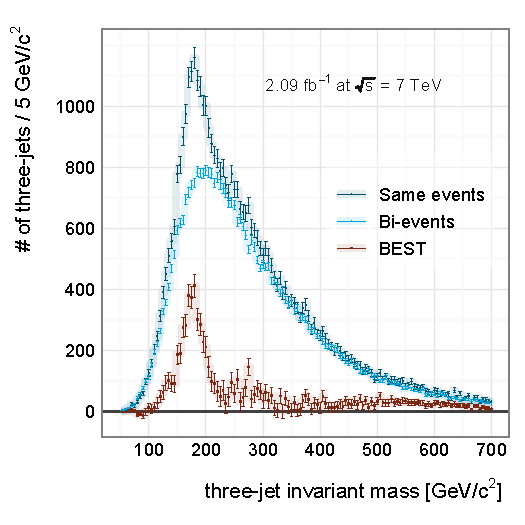
\includegraphics[scale=1.]{figs/best/c110506_s0102_g002_01}
  \caption{The invariant mass distributions of three jets with one
  b-tagged in the same events, bi-events, and BEST events in 2.09
  fb${}^{-1}$ of data. Events were triggered by muons and selected to
  choose top-antitop pair production events} \label{151919_8Aug11}
 \end{center}
\end{figure*}

\begin{figure*}[!h]
 \begin{center}
  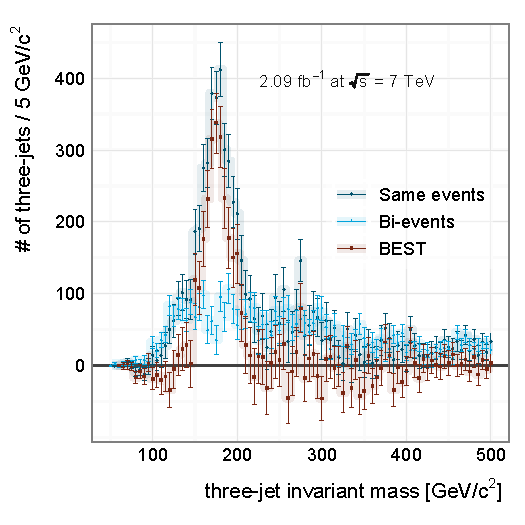
\includegraphics[scale=1.]{figs/best/c110506_s0102_g004_01}
  \caption{The invariant mass distributions of three jets with one
  b-tagged in the same events, bi-events, and BEST events after the 2nd
  BEST in 2.09 fb${}^{-1}$ of data. Events were triggered by muons and
  selected to choose top-antitop pair production events}
  \label{095120_31Dec11}
 \end{center}
\end{figure*}

\begin{figure*}[!h]
 \begin{center}
  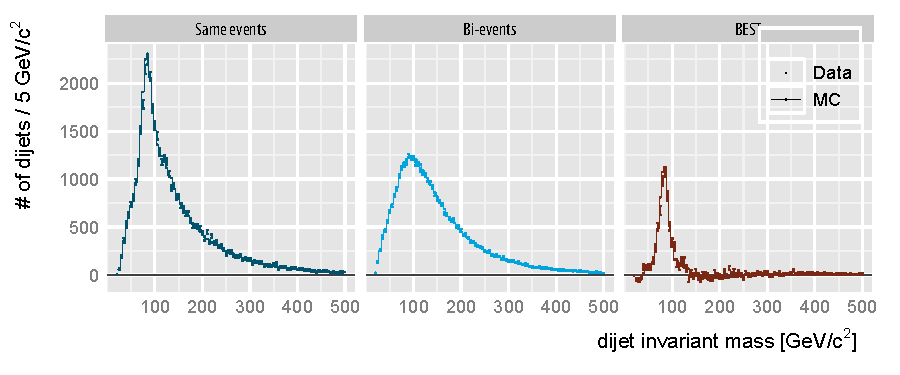
\includegraphics[scale=1.]{figs/best/c110506_s0102_g021_01}
 \caption{The data-MC comparisons of the distributions in Fig. \ref{153631_13Aug11}}
 \label{100843_31Dec11}
 \end{center}
\end{figure*}

\begin{figure*}[!h]
 \begin{center}
  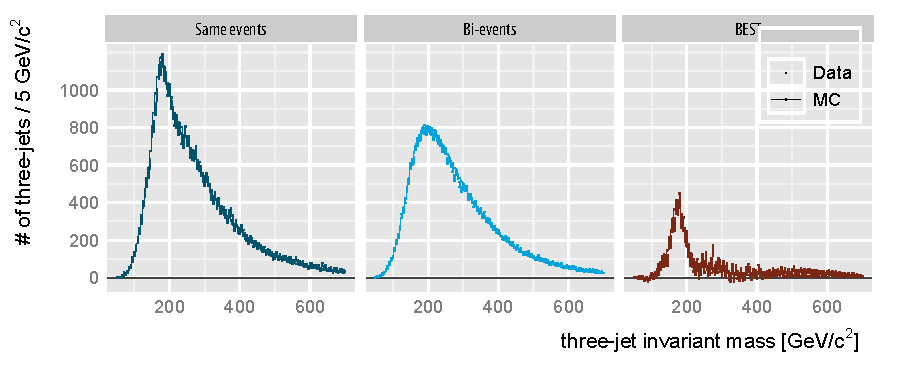
\includegraphics[scale=1.]{figs/best/c110506_s0102_g022_01}
 \caption{The data-MC comparisons of the distributions in Fig. \ref{151919_8Aug11}}
 \label{100851_31Dec11}
 \end{center}
\end{figure*}

\begin{figure*}[!h]
 \begin{center}
  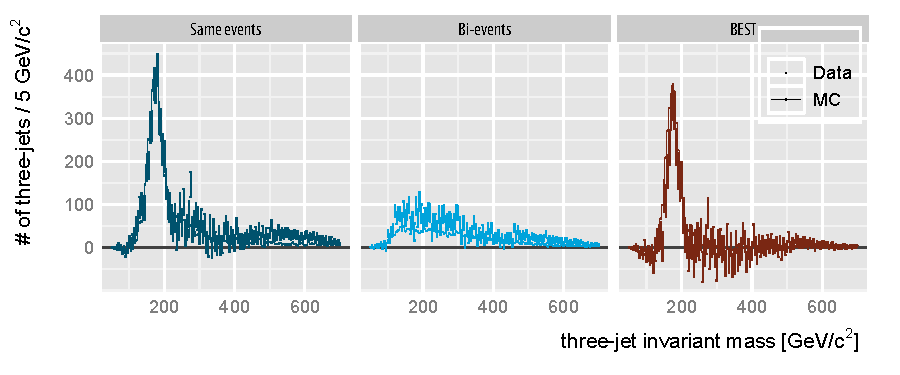
\includegraphics[scale=1.]{figs/best/c110506_s0102_g024_01}
 \caption{The data-MC comparisons of the distributions in Fig. \ref{095120_31Dec11}}
 \label{100859_31Dec11}
 \end{center}
\end{figure*}

Fig. \ref{100843_31Dec11}, Fig. \ref{100851_31Dec11} and Fig.
\ref{100859_31Dec11} show the data-MC comparisons of the distributions
respectively in Fig. \ref{153631_13Aug11}, Fig. \ref{151919_8Aug11}, and
Fig. \ref{095120_31Dec11}. \textit{TTJets\_TuneZ2\_7TeV-madgraph-tauola}
was used for MC.


Fig. \ref{101357_31Dec11} and Fig. \ref{101404_31Dec11} show the MC
closure tests for invariant mass of respectively dijets and three-jets.

\begin{figure*}[!h]
 \begin{center}
  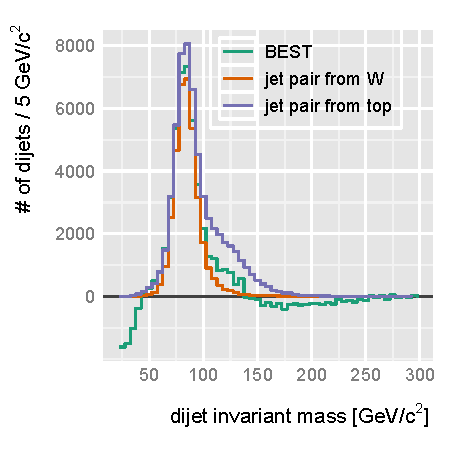
\includegraphics[scale=1.]{figs/best/c110506_s0102_g031_02}
 \caption{MC closure: the invariant mass distributions of dijets in the
 BEST events, dijets from the same W bosons, dijets from the same top
 quarks}
 \label{101357_31Dec11}
 \end{center}
\end{figure*}

\begin{figure*}[!h]
 \begin{center}
  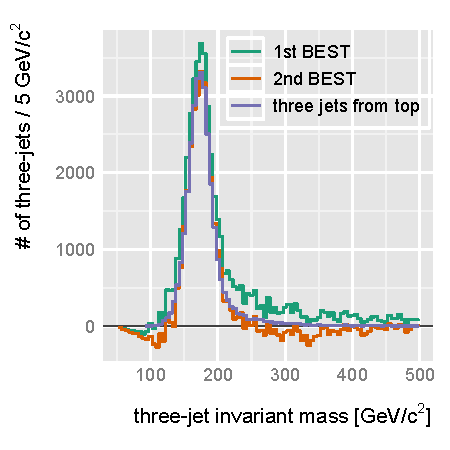
\includegraphics[scale=1.]{figs/best/c110506_s0102_g041_02}
 \caption{MC closure: the invariant mass distributions of three-jets in
  the 1st BEST event, the 2nd BEST events, and the three-jets from the
  same top quarks}
 \label{101404_31Dec11}
 \end{center}
\end{figure*}
